	
\subsubsection{03.11.14}

\begin{enumerate}
	\item Время начала и окончания собрания:\newline
	14:00 – 21:40
	\item Цели собрания:\newline
	\begin{enumerate}
	  \item	Завершить работу над механизмом лебедки.\newline
	  
	  \item	Установить драйвер приводов для лебедки.\newline
	  
	  \item	Написать программу для управления лебедкой.\newline
	  
	  \item	Закрепить ремень с помощью ниток.\newline
	  
    \end{enumerate}
    
	\item Проделанная работа:\newline
	\begin{enumerate}
	  \item	Драйвер приводов был установлен на робота.\newline
      
      \item	Приводы были соединены между собой катушкой, на которую будет наматываться ремень.\newline
      
      \item	Ремень был надежно пришит к последней перекладине с одной стороны и к катушке лебедки с другой.\newline
      
      \begin{figure}[H]
      	\begin{minipage}[h]{0.47\linewidth}
      		\center{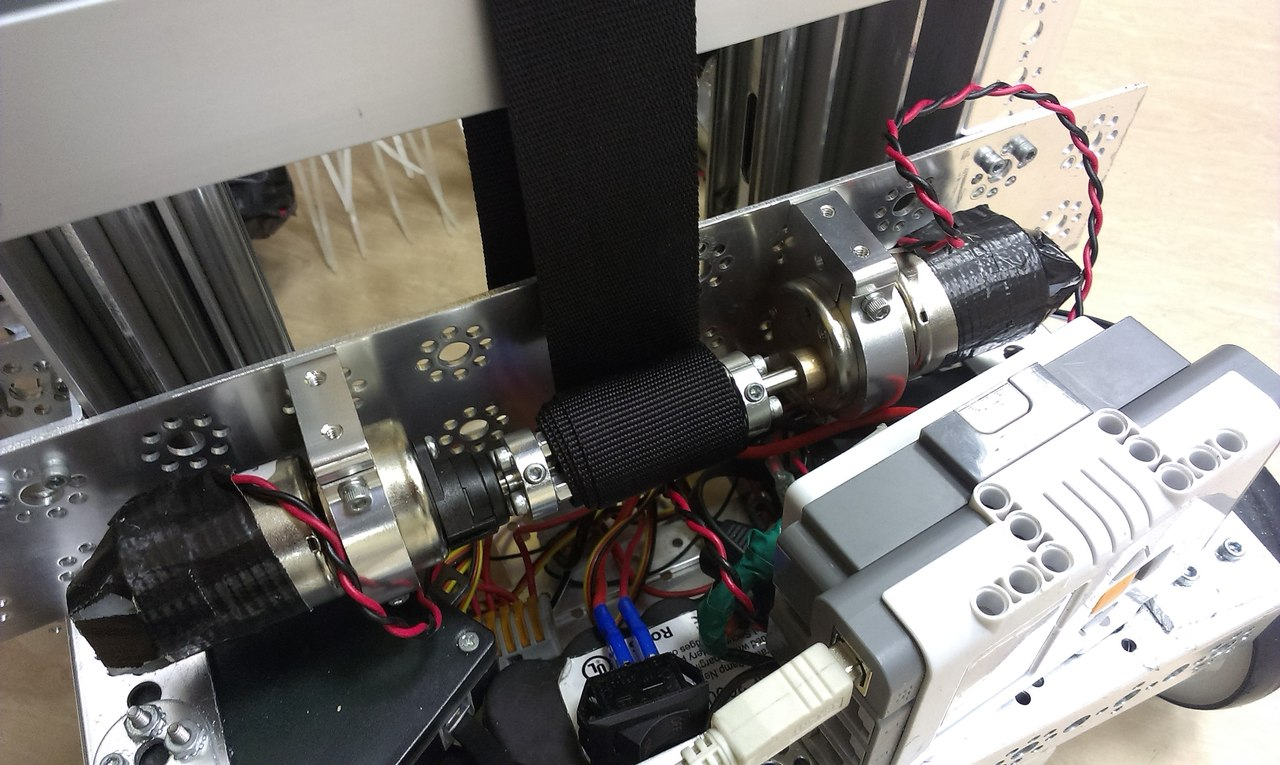
\includegraphics[width=1\linewidth]{days/images/jMNEE3KITgc}}
      		\caption{Лебедка}
      	\end{minipage}
      	\hfill
      	\begin{minipage}[h]{0.47\linewidth}
      		\center{
\includegraphics[width=1\linewidth]{days/images/missing_image}}
      		\caption{Ремень закреплен нитками}
      	\end{minipage}
      \end{figure}
      
      \item	Для испытания подъемника была написана простейшая программа, позволявшая лебедке вращаться с максимальной скоростью в каждую сторону либо стоять неподвижно. Движение лебедки контролировалось с помощью правого аналогового датчика.\newline
      
      \item	Во время испытания подъемника было обнаружено, что валы приводов расположены не соосно, из-за чего в процессе работы вся конструкция лебедки ужасно шаталась. Несмотря на это, лебедка была в состоянии раздвигать подъемник. Тем не менее, было решено изменить конструкцию лебедки таким образом, чтобы катушка располагалась на отдельной оси, усилие на которую передавалось бы с приводов через шестеренки с передаточным отношением 1:1. Это позволило бы устранить проблемы, связанные с несоосным расположением валов приводов.\newline
      
      \item	Для того, чтобы лебедка не сломала подъемник, продолжая работать после того, как он раздвинется на максимальную высоту, было решено установить ограничения на ее движение. Для этого было решено на следующем занятии установить на один из приводов лебедки энкодер и написать программу, считывающую его показания и устанавливающую нижнюю и верхнюю границы движения лебедки.\newline
      
    \end{enumerate}
    
	\item Итоги собрания: \newline
	\begin{enumerate}
	  \item	Драйвер приводов установлен на робота.\newline
	  
	  \item	Ремень надежно закреплен на механизме подъемника и лебедки.\newline
	  
	  \item	Проведены испытания лебедки. Выяснено, что два привода имеют достаточно мощности для раздвигания подъемника.\newline
	  
    \end{enumerate}
    
	\item Задачи для последующих собраний:\newline
	\begin{enumerate}
	  \item	Переделать конструкцию лебедки так, чтобы она была более надежной.\newline
	  
	  \item Подсоединить энкодер к одному из приводов лебедки и добавить в программу ограничения движения лебедки.\newline
	  
    \end{enumerate}     
\end{enumerate}

\fillpage
